% !TeX spellcheck = de_DE

\chapter{Prinzipien der OTA-Updates}
\label{sec:princip}
Aufgrund des schnellen Tempos mit dem sich das IoT entwickelt und die ständig steigenden Zahlen der IoT Geräte, besteht ein zunehmender Bedarf, Software-Updates für Sicherheitsaspekte, Fehlerkorrekturen und Software-Erweiterungen zu unterstützen. Für die kleinsten IoT-Geräte ist es zu aufwändig, die Updates mittels angeschlossener USB-Leitung hochzuladen und auszuführen. Deshalb wird eine Softwareaktualisierung über eine Funkschnittstelle (typischerweise WLAN oder Mobilfunknetz) durchgeführt, somit können sogar die in Wänden verbauten Geräte erreicht werden. Der englische Begriff "Over-the-Air-Update" (OTA) bedeutet "Aktualisierung über Luft". Diese Technologie hat bereits eine historische Entwicklung hinter sich. Zu Beginn der 2000er Jahre war es gewöhnlich SMS-Nachrichten mit Bildern an das Telefon zu senden oder mit SMS einen kostenpflichtigen Bildschirmschoner zu bestellen. Zu diesem Zweck musste ein spezieller digitaler Code, der aus dem Katalog ausgewählt wurde, an eine kurze Nummer gesendet werden. Siemens-Telefone gehörten damals mit ihrem „Siemens OTA“ zu den Pionieren, der als Standard für die Übertragung nicht nur von Bildern und Bildschirmschonern, sondern auch von WAP-Einstellungen, Kontakten, Kalenderereignissen usw. konzipiert wurde.

Das OTA Update ist praktisch der Industriestandard für die Aktualisierung von Software auf einem mobilen Gerät. Jedoch sind reine OTA Updates in ihrer Funktionalität zu begrenzt. Es war nur die manuelle Installation von Konfigurationsprofilen zulässig, es konnten keine neuen Profile automatisch gepullt werden; die Geräte und seine Sicherheitseinstellungen konnten nicht automatisch aktualisiert werden, es gab keine Befehle zu Verfügung. Heutzutage ist OTA mit der Verwendung vom größeren Geräteverwaltungssystems MDM (Device Management System) verstärkt, das einen Standort des IoT-Geräts und den Status des Updates überwacht und somit unter anderem das Aktualisieren von Software oder die Konfiguration des IoT-Geräts ermöglicht. Auf der Geräteseite kommuniziert OTA-/DM-Klient mit dem Server. Viele MDM-Anbieter verwenden OTA zum Herunterladen und Installieren eines Konfigurationsprofils mit MDM-Nutzdaten auf einem Gerät und später eine installierte MDM für die weitere Geräteverwaltung.

Zunächst muss ein Hersteller der Software in der Lage sein, gleichzeitig z.B. über den seriellen oder USB-Anschluss den Bootloader und die ursprüngliche Firmware auf dem IoT-Gerät zu flashen. Die anfängliche Firmware enthält normalerweise ein Softwaremodul für Firmware-Updates, das mit der erforderlichen Vertrauensbasis des Betreuers konfiguriert ist. Das OTA-Modell basiert auf einer einzelnen Vertrauensbasis (Root of Trust), mit der die Authentizität des signierten Firmware-Images überprüft wird. Wenn es bei einem Angriff gelingt, den privaten Schlüssel zu bekommen, der dem Stamm des Vertrauens zugeordnet ist, können Angreifende schädliche Firmware-Images auf das IoT-Gerät laden. Softwarenentwickler*innen können ein neues Firmware-Image und die entsprechenden Metadaten erstellen, die mit dem privaten Schlüssel des Softwareentwicklers signiert sind. Die Firmware und die signierten Metadaten können dann auf den IoT-Softwareupdate-Server hochgeladen werden. Die Hauptaufgaben des IoT-Update-Moduls bestehen darin, sowohl das Firmware-Image vom Update-Server abzurufen, die Metadaten zu analysieren und zu überprüfen als auch das Firmware-Image im Flash-Speicher zu speichern. Die Metadaten beschreiben Firmware-Updates und bieten Informationen zur Firmware, die zum Aktualisieren des Geräts erforderlich ist. Die empfangenen Metadaten werden mithilfe des Vertrauensankers (des auf dem Gerät gespeicherten öffentlichen Schlüssels) kryptografisch überprüft. Wenn die digitale Signatur überprüft wird und andere Sicherheitsüberprüfungen bestanden werden (z. B. wird bestätigt, dass die Firmware-Sequenznummer neuer ist), schreibt das Modul auch die Metadaten in den Flash (andernfalls werden die Metadaten ausgeblendet) und ein Neustart wird eingeleitet. Der Bootloader wählt dann die neue gültige Firmware basierend auf den Metadaten. Das IoT-Firmware-Update Szenario ist auf der Abbildung \ref{fig:ota} zu sehen \cite[p.5]{website:SecureFirmware}.

\begin{figure}[h!]
	\centering
	\fbox{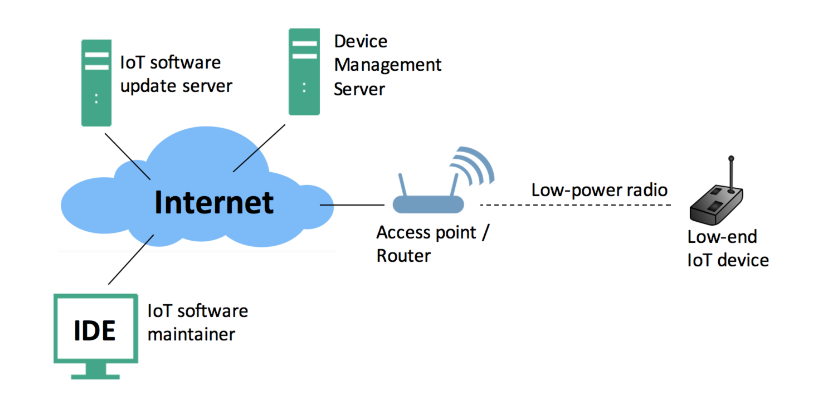
\includegraphics[width=1\textwidth]{gfx/ota.png}}
	\caption{IoT-Firmware-Update Szenario}
	\label{fig:ota}
\end{figure}


Die Software auf einem IoT-Gerät muss darauf vorbereitet sein, einen Aktualisierungsmechanismus zu unterstützen. Das Gerät benötigt einen Bootloader, die Logik, die beim Booten des Geräts zuerst ausgeführt wird und bestimmt, welche Firmware es startet. Manchmal sind Geräte mit mehreren Bootloadern ausgestattet. Zum Beispiel ein Bootloader der Stufe 1 im ROM und ein Bootloader der Stufe 2, die aktualisiert werden können. Der Grund für solche Designs ist sicherheitsrelevant, da das Aktualisieren eines Bootloaders zu einem unsicheren Gerät führen kann. Immer wenn ein Bootloader auf einem Gerät vorhanden ist, muss das Speicherlayout der Hardware berücksichtigt und die Ausnahmebehandlungsroutinen neu positioniert werden \cite[p.3]{website:SecureFirmware}.

Der typische Ansatz für IT-Software-Updates besteht darin, das vollständige Firmware-Image sofort zu ersetzen. Der Vorteil der Aktualisierung der vollständigen Firmware liegt in der Einfachheit dieses Ansatzes. Die Verwendung modernster kryptografischer Algorithmen ist erforderlich, um die Sicherheit von Firmware-Aktualisierungen zu gewährleisten. Sie können bei Bedarf auch während der neuen Konfiguration des Gerätes aktualisiert werden. 

\chapter{Grundlagen der Sicherheitsaspekten}
\label{sec:sicher}
Viele IoT-Geräte erfordern die Erfassung, Analyse und Übertragung potenziell sensibler Daten. Es ist wichtig, dass diese Daten jederzeit angemessen geschützt sind und Benutzer*innen wissen, welche privaten Daten verarbeitet werden. Sicherheitsarchitekturen für Geräte, Netzwerke und Systeme sollten gleichzeitig mit den Geräten selbst entwickelt und nicht zu einem späteren Zeitpunkt nachgerüstet werden. Neben dem Gerät selbst können sensible Daten in anderen verbundenen Systemen verfügbar gemacht werden \cite[p.5]{website:Principles}. Der Prozess, wie die Sicherheit der Daten im gesamten Netzwerk aufrechterhalten wird, muss berücksichtigt werden. Die Verhinderung des unbefugten Zugriffs oder der unbefugten Kontrolle ist für die Sicherung von Geräten von entscheidender Bedeutung. Wenn bei einem Angriff die Kontrolle über das Gerät erlangt wird, kann möglicherweise auf vertrauliche Daten zugegriffen oder an anderer Stelle im Netzwerk Probleme verursacht werden. \cite[p.11]{website:Principles}. Es ist notwendig, die Software auf dem Gerät zu aktualisieren, da eine veraltete Software möglicherweise nicht gepatchte Sicherheitslücken enthält. Solche Sicherheitslücken können die Ausnutzung des Geräts und seiner Daten durch einen Angriff ermöglichen. Sicherheitspatches / -updates sollten rechtzeitig angewendet werden, ohne die Funktionalität des Geräts zu beeinträchtigen. Durch das Zulassen nicht authentifizierter Updates kann bei einem Angriff möglicherweise schädlicher Code auf dem Gerät ausgeführt werden \cite[p.12]{website:Principles}.

\section{Einschränkungen der Bescheinigungs-Verfahren}
\label{sec:sicher:tpm}
Die Bescheinigung ist eine Interaktion zwischen zwei Parteien, bei der die prüfende Partei den aktuellen Zustand und /oder das Verhalten der zu prüfenden Seiten feststellt \cite[p.11]{website:Attestation}. Ziel der Bescheinigung ist es, einer dritten Partei zu beweisen, dass das Betriebssystem und Ihre Anwendungssoftware intakt und vertrauenswürdig sind. In diesem Kapitel werden die Einschränkungen der klassischen Bescheinigung-Verfahren kurz analysiert: das Trusted Platform Module (TPM) und die softwarebasierte Bescheinigung. 

TPM ist eine sichere kryptographische Hardware, die auf der Systemplatine integriert ist und primitive kryptografische Funktionen implementiert, auf denen komplexere Funktionen aufgebaut werden können. Die prüfende Partei vertraut darauf, dass die Bescheinigungsdaten korrekt sind, da sie von einem TPM signiert sind, dessen Schlüssel von der Zertifizierungsstelle (CA) zertifiziert ist \cite[p.4]{website:TPM}. Jedoch hat der Bescheinigungsprozess einige Einschränkungen. Zwar kann durch eine Bescheinigung der prüfende Partei zuverlässig mitgeteilt werden, welche Anwendungen auf einem Clientcomputer ausgeführt werden, aber die prüfende Partei muss weiterhin beurteilen, ob jede bestimmte Software vertrauenswürdig ist \cite[p.7]{website:TPM}. Die Entscheidung, einer bestimmten Software zu vertrauen, basiert oft auf einer weißen Liste von Software, die als vertrauenswürdig bekannt ist. Eine schwarze Liste könnte leicht unüberschaubar groß werden. Das Prüfen der Software auf Sicherheit und das Verwalten einer Datenbank mit vertrauenswürdigen Anwendungen ist keine triviale Aufgabe \cite[p.7]{website:TPM}.

In IoT kann TPM-Bescheinigung auf der Ebene des Endgerätes nicht verwendet werden. Für die Implementierung wird zusätzliche Hardware benötigt, was im Fall der kleinsten IoT-Geräte nicht gewünscht ist, da damit die Größe der Endgerät vergrößert und mehr Strom verbraucht wird. Meistens muss mindestens das Doppelte des Speicherplatzes auf dem aktualisierten Gerät  bereitgestellt werden. Wenn ein Rollback-Mechanismus erforderlich ist, ist mindestens dreimal so viel Speicherplatz erforderlich - einmal für die laufende Anwendung, einmal für die neue Firmware und einmal für die Rollback-Firmware. Der Vorteil auf der anderen Seite ist, dass ein solches Gerät durch ein fehlerhaftes Firmware-Update oder sogar durch eine Unterbrechung während des drahtlosen Updates nur sehr schwer zu blockieren ist. Somit erhöht die TPM-Bescheinigung auch die Hardwarekosten für die TPM-Integration \cite[p.17]{website:Attestation}. Zusammenfassend kann man sagen, dass TPM-Bescheinigung nur das anfängliche Laden von Software abdeckt und mit einer Prüfung nur ein Endgerät behandelt. Somit ist die "Entscheidung über die Vertrauenswürdigkeit" nicht skalierbar, da die Messungen für die Zuverlässigkeit sich mit jedem Software-Update ändert. 

Die Root of Trust berechnet einen Hash-Wert des geladenen Speichers und vergleicht diesen mit einem signierten Wert. Ein Gerät darf nur dann hochfahren, wenn alle Prüfungen bestanden wurden. Das Problem mit der statischen Vertrauensbasis besteht darin, dass sie im Allgemeinen keine Garantie für den aktuellen Status eines Geräts bietet, da nach dem Start die vorhandene Malware die Daten fälschen kann. Noch schlimmer ist, dass eine statische Vertrauenswurzel (z. B. TPM v1.1 oder Secure Boot) nicht zum Erkennen einiger Klassen leistungsfähiger Angriffe geeignet ist.

Die softwarebasierte Bescheinigung verspricht, die Integritätsprüfung zu ermöglichen, ohne dass eine bestimmte Hardware erforderlich ist. Bestehende Vorschläge können jedoch Sicherheit schwächen. Zum Beispiel mit der Verwendung von maximalen Netzwerk-Roundtrip-Zeit zum Definieren des Attestierungs-Timeouts, währenddessen ehrlichen Geräten rechtzeitig antworten dürfen. In einem Szenario von Internet der Dinge ist es nicht anwendbar, da die zahlreichen Geräte über ein an sich unzuverlässiges drahtloses Medium kommunizieren müssen. Darüber hinaus erfordert ein größeres Zeitlimit mehr Berechnungen, die zusätzliche Zeit und Energie verbrauchen und das Gerät von der Ausführung seiner Hautaufgaben abhält \cite{website:softAtt}. 

\section{Hybridbescheinigung: SMART}
\label{sec:sicher:smart}
Wie bereits erwähnt wurde, umfassen hardwarebasierte Ansätze die Sicherheits-Co-Prozessoren, die für eingebettete Low-End-Geräte zu teuer sind. Gleichzeitig haben frühere softwarebasierte Techniken keine konkreten Sicherheitsgarantien geboten. Ein neuer sicherer Ansatz namens SMART konzentriert sich auf den Aufbau einer dynamischen Vertrauensbasis in einem Remote-Embedded-Gerät auf Low-End-Mikrocontroller-Einheiten (MCU), denen spezielle Speicherverwaltungs- oder Schutzfunktionen fehlen. Dies bietet eine Möglichkeit, die Bescheinigung nach dem Booten dynamisch durchzuführen. Dies wird erreicht, indem ein bestimmter CPU-Befehl gestattet wird, den Status einiger PCRs atomar zurückzusetzen, Speicherbereiche zu isolieren, den Inhalt dieses Speichers zu hashen und auszuführen \cite[p.12]{website:smart}. 

Im Design ist es vorgesehen, dass das zu überprüfende Gerät (PRV) und Prüfer (VRF) einen gemeinsamen geheimen Schlüssel haben. Schließlich wird es angenommen, dass der Schlüssel  nur von dem Read-Only-Attestierungsspeicher Region aufgerufen werden darf. Der Zugriff darauf ist nur über SMARTcode im ROM möglich, der nicht nur den Zugriff auf K steuert, sondern auch verhindert, dass Nicht-SMARTcode darauf zugreift. Wenn ein Fehler von Sicherheitskomponenten gemeldet wird, wird ein Hardware-Reset der MCU durchgeführt. Beim Zurücksetzen erzwingt die Hardware eine Speicherbereinigung.


Der geheime Schlüssel kann in der PRV während der Produktionszeit oder später vorinstalliert werden. Eine nicht verschlüsselte Funktion, wie beispielsweise ein kryptografischer Hash (z. B. SHA-256), ist für die Prüfung ungeeignet. Dies liegt daran, dass jeder ohne einen geheimen Schlüssel einen Hash einer Eingabe berechnen und eine Antwort von PRV fälschen kann. Dies kann insbesondere Malware tun, die PRV infiziert hat. Daher wird die kryptografische Prüfsumme als HMAC mit K-Schlüssel implementiert, der sich in einem sicheren Speicher auf der MCU von PRV befindet. Die Verwendung von und der Zugriff auf K wird von der MCU so eingeschränkt, dass nur vertrauenswürdiger und unveränderlicher SMART ROM Code (RC) es verwenden darf. RC verwendet seinerseits nur K, um HMAC zu berechnen, und übergibt dann die Kontrolle an Code to Attest (HC). SMART berechnet einen HMAC eines bestimmten Speichersegments und springt dann - ohne unterbrochen zu werden - zu einer vom Prüfer angegebenen Adresse innerhalb dieses Segments. Die Implementierung besteht aus ungefähr 500 Zeilen C-Code, was die Überprüfung der Richtigkeit sowohl machbar als auch relativ einfach macht.\cite[p.4]{website:smart} 

Der für die Berechnung des HMAC verwendete Schlüssel kann nicht im normalen Speicher gespeichert werden, da Malware leicht auf die Bescheinigung zugreifen und diese bestätigen kann. Ein spezieller hardwaregesteuerter Speicherort ist für einen einzelnen symmetrischen Schlüssel K vorgesehen. Dieser Speicher muss gegen Software-Angriffe immun sein. Hardware-Angriffe werden im Rahmen dieser Arbeit nicht betrachtet, da dafür ein direkter physischer Zugriff oder zumindest eine sehr enge physische Nähe zum Zielgerät erforderlich ist. Dies ist in vielen Einstellungen mit eingeschränktem Zugriff unwahrscheinlich \cite[p.6]{website:smart}. Zur K-Geheimhaltung wird sichergestellt, dass auf den Schlüssel nur zugegriffen werden kann, wenn sich der Programmzähler (PC) im RC-Speicherbereich befindet. Es wird folgendes angenommen: K steht der vertrauenswürdiger Software nicht direkt zur Verfügung. Wenn ein Fehler auftritt, wird die Ausführung gestoppt und es werden keine Informationen über K rausgegeben. Seitenkanäle können nicht zum Sammeln von Informationen über nicht vertrauenswürdige Software verwendet werden, die auf der MCU ausgeführt wird \cite[p.8]{website:smart}. 

Die natürlichste Verwendung von SMART besteht darin, ein Speichersegment zu bestätigen und zu überprüfen, ob es Daten (oder Code) enthält, die es voraussichtlich enthalten muss. Mit dem Algorithmus kann sichergestellt werden, dass ein Gerät erfolgreich zurückgesetzt wurde. Es kann zur Sicherstellung verwendet werden, dass die von einem Peripheriegerät gelesenen Werte nicht durch möglicherweise auf diesem Gerät vorhandene Malware gefälscht werden können.

Die Autoren von SMART zeigen, dass eine einfache Messroutine im ROM mit exklusivem Zugriff auf einen geschützten geheimen Schlüssel es ermöglichen kann, eine Remote-Bestätigung und eine vertrauenswürdige Ausführung zu implementieren \cite{website:smart}. SMART löst jedoch nicht das Problem der Behandlung von Speicherzugriffsverletzungen und Hardware-Interrupts, sondern verlässt sich auf die Plattform, um die CPU zurückzusetzen und den gesamten Speicher zu bereinigen. Darüber hinaus unterstützt die eher grundlegende Zugriffssteuerungslogik von SMART weder die Aktualisierung des Bestätigungscodes noch dessen Schlüssel, und die Interaktion zwischen mehreren geschützten Modulen ist sehr langsam \cite[p.2]{website:TrustLite}. Deshalb werden die weiteren Sicherheitsalgorithmen für IoT betrachtet.

\section{Hybridbescheinigung: TrustLite und TyTAN}
\label{sec:sicher:trust}
TrustLite bietet eine generische Sicherheitsarchitektur für kostengünstige eingebettete Systeme, bei denen die Hardware- und Softwareumgebung sehr dynamisch ist und bei denen die Kosten für sichere Betriebssysteme oder den Hardwareschutz ein wesentlicher Faktor sind. Wie bei den meisten eingebetteten Geräten wird davon ausgegangen, dass die CPU von einem festverdrahteten, bekannten Standort im nichtflüchtigen Speicher wie dem programmierbaren ROM (PROM) startet und dass jeder Peripheriezugriff mit zugeordnetem Speicher (MMIO) implementiert wird \cite[p.3]{website:TrustLite}. 

TrustLite wird mit einer strengen Datenisolierung entwickelt, d.h. dass keine andere Software auf der Plattform den mit TrustLite gesicherten Code ändern kann. Trustlet-Daten können von anderen Trustlets gemäß der Systemrichtlinie gelesen oder geändert werden. Der lokalen Zustand des Plattform kann vom TrustLite überprüft und validiert werden, ohne dass andere Software in der Lage ist, das Verfahren zu manipulieren. Ein schneller Start ist vorgesehen, sodass die Sicherheitserweiterungen die Bootstrapping-Verzögerung nicht wesentlich beeinflussen sollten, z.B. indem sie große Codemengen messen oder kryptografische Operationen bei der Plattform- oder Trustlet-Initialisierung durchführen. Zusätzlich zum vertrauenswürdigen SoC ist ein Secure Loader dafür verantwortlich, alle gewünschten Trustlets und ihre kritischen Datenbereiche in den On-Chip-Speicher zu laden. Darüber hinaus programmiert es die MPU, um die Trustlet-Speicherbereiche sowie ihre eigenen Codean- und Datenbereiche vor unbefugtem Zugriff zu schützen \cite[p.4]{website:TrustLite}. 

Die TrustLite-Sicherheitsarchitektur sollte kurz beschrieben werden. Die konfigurierten Code- und Datenbereiche werden in der schreibgeschützten Tabelle im On-Chip-Speicher gespeichert, sodass sie von einzelnen Trustlets oder Attestierungsroutinen nachgeschlagen und validiert werden können. Nur dann lädt der Secure Loader weiterhin nicht vertrauenswürdige Software wie das eingebettete Betriebssystem und führt sie aus. Secure Loader selbst ist nur zur Initialisierungszeit aktiv. Es konfiguriert nur den Hardware-Speicherschutz und initialisiert optional eine Vertrauenskette für die Remote-Bestätigung und die vertrauenswürdige Ausführung, bevor die Steuerung an den tatsächlichen Laufzeitcode delegiert wird, z. B. an ein nicht vertrauenswürdiges Betriebssystem \cite[p.4]{website:TrustLite}. 

Wenn die MPU eine Speicherschutzverletzung erkennt, wird eine CPU-Ausnahme ausgelöst und wie bei normalen MPU-Designs behandelt. Bei der Behandlung von CPU-Ausnahmen wie Fehlern, Traps und Interrupts führen typische Computerplattformen nur die minimalen Aufgaben des Speicherns des Stapels und des Befehlszeigers aus, bevor der entsprechende (Software-) Ausnahmebehandler ausgeführt wird. Dieses Verfahren öffnet jedoch Trustlets für Angriffe auf Daten/Informationen. Im Folgenden ist mit der Verwendung von TrustLite eine modifizierte CPU-Ausnahme-Engine vorgeschlagen, die die Speicherisolation von Aufgaben auch bei Hardware- und Software-Ausnahmen behandeln kann \cite[p.6]{website:TrustLite}. Um die Isolierung von Trustlets angesichts nicht vertrauenswürdiger ISRs zu gewährleisten, wird das Standardschema zum Speichern des Stapelzeigers, des Befehlszeigers und der CPU-Flags zusammen mit zusätzlichen Ausnahmeinformationen auf dem Betriebssystem geändert. Die Hardware-Ausnahmemaschine speichert zuerst den CPU-Status im aktuellen Stapel-SPA, speichert dann den SPA in der Trustlet-Tabelle und löscht dann alle Allzweckregister. Erst dann wird der OS-Stapelzeiger wiederhergestellt und der reguläre Betrieb der Ausnahme-Engine kann fortgesetzt werden, indem der fehlerhafte IP-Wert sowie zusätzliche Fehlercodes auf den neuen Stapel-SPOS geschrieben werden \cite[p.9]{website:TrustLite}.

\begin{figure}[h!]
	\centering
	\fbox{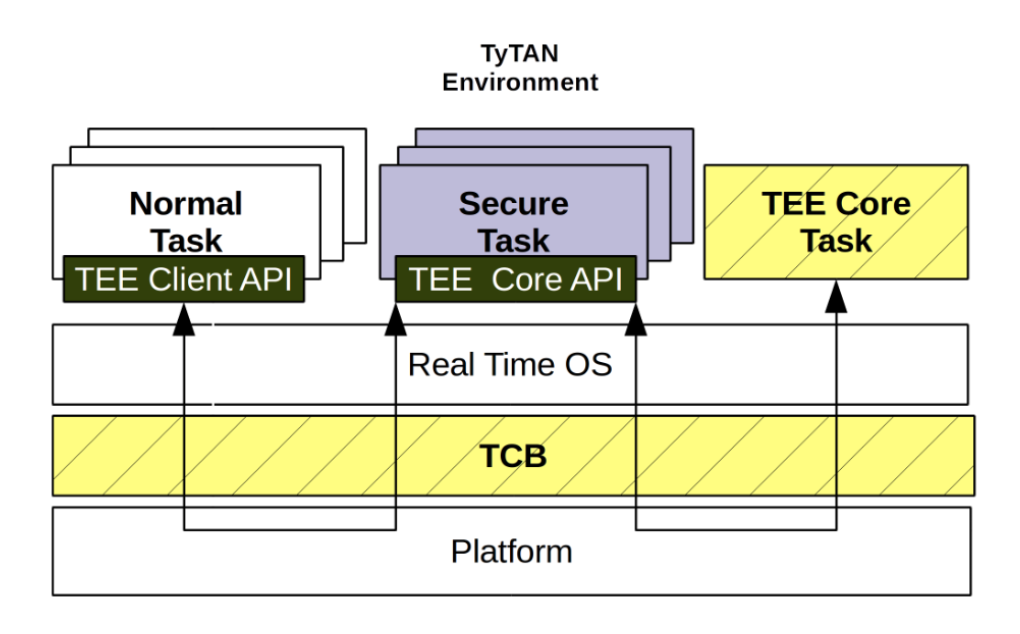
\includegraphics[width=0.7\textwidth]{gfx/tytan.png}}
	\caption{TyTAN Architekturdiagramm}
	\label{fig:tyt_arch}
\end{figure}

TyTAN ist die Sicherheitsarchitektur für eingebettete Systeme, die eine hardwareunterstützte, starke Isolierung dynamisch konfigurierbarer Aufgaben und Echtzeitgarantien bietet. Durch in TrustLite eingeführte Hardwarefunktionen sowie Echtzeit-Planungsgarantien bietet TyTAN eine starke Isolierung dynamisch konfigurierbarer Aufgaben. Es wird auch die sichere Ausnahme-Engine von TrustLite verwendet, um einen sicheren IPC-Mechanismus (Inter Process Communication) bereitzustellen, bei dem sowohl Sender als auch Empfänger anhand der Zusammenfassung der jeweiligen Aufgaben authentifiziert werden können, die beim Laden gemessen werden. Vergleichend zu TrustLite ist hier dynamische Konfiguration interessant. Aufgaben (Anwendungen) können dynamisch geladen, entladen, gestartet und bei Bedarf zur Laufzeit gestoppt werden, wodurch die Effizienz durch eine bessere Nutzung der Ressourcen erhöht wird. Aufgaben können aktualisiert werden, um Softwarefehler zu beheben. TyTAN unterstützt zwei Arten von Aufgaben: Normale Aufgaben sind von anderen Aufgaben isoliert, aber für das Betriebssystem zugänglich; sichere Aufgaben, die von allen anderen Softwareprogrammen einschließlich des Betriebssystems isoliert sind \cite[p.2]{website:TyTAN}. Die TyTAN Architektur ist auf der Abbildung \ref{fig:tyt_arch} zu sehen. Die TyTAN-Hardwareplattform wird mit einem Plattformschlüssel Kp geliefert. Der Zugriff auf diesen Schlüssel wird von der MPU gesteuert und nur vertrauenswürdige Softwarekomponenten haben Zugriff darauf. Die vertrauenswürdigen Softwarekomponenten von TyTAN werden mit einem sicheren Start geladen und von der MPU vom Rest des Systems isoliert, um ihre Integrität sicherzustellen. Um die Integrität einer Aufgabe gegenüber einem lokalen oder Remote-Prüfer zu beweisen, berechnet die RTM (Root of Trust for Measurement) mithilfe einer kryptografischen Hash-Funktion den Hash-Wert für den Binärcode jeder erstellten Aufgabe. Um die Echtzeitanforderungen zu erfüllen, muss die RTM während der Hash-Berechnung unterbrechbar sein. Für sichere Aufgaben gibt es zwei Einschränkungen: (1) Das Betriebssystem kann nicht auf den Stapel einer sicheren Aufgabe zugreifen und deren Kontext wiederherstellen. und (2) sichere Aufgaben können nur mit einer dedizierten Eintragsroutine aufgerufen werden \cite[p.3]{website:TyTAN}. 

Das Hauptziel von TyTAN ist die Gewährleistung der Integrität kritischer Softwarekomponenten und sicherer Aufgaben. Dies wird durch einen sicheren Start und eine durch Hardware erzwungene Speicherzugriffskontrolle erreicht. Eine weitere wichtige Eigenschaft von TyTAN ist die Echtzeitausführung von Aufgaben, die von der Verfügbarkeit der Plattform abhängt \cite[p.4]{website:TyTAN}.

%=========================================

\chapter{Standards für die Remote-IoT-Geräteverwaltung}
\label{sec:ota}

Ein wichtiger Aspekt von IoT-Firmware-Updates betrifft die Verbreitung von Software über das Netzwerk. In dieser Arbeit werden das Standardprotokoll MQTT und den bekannteste offene Standard LwM2M betrachtet. 

\section{MQTT-Protokoll}
\label{sec:ota:mqtt}
MQTT (Message Queuing Telemetry Transport) hat das Internet der Dinge stark beeinflusst, da es leicht und robust ist und es ermöglicht, die Verbreitung von Software-Updates an eine Menge von IoT-Geräten gleichzeitig auszuführen. Die Verwendung von MQTT über SSL bedeutet eine Kommunikation zwischen den Edge-Knoten und dem Cloud-Backend. MQTT verwendet eine themenbasierte Publish-Subscribe-Architektur. Dies bedeutet, dass, wenn ein Client eine Nachricht M zu einem bestimmten Thema T veröffentlicht, alle Clients, die das Thema T abonniert haben, die Nachricht M erhalten \cite{website:mqttcoap}. Vergleichend zu HTTP ist MQTT schneller, da die HTTP-Anforderung die Verbindung bei jeder Anforderung öffnet und schließt, während MQTT online bleibt, damit der Kanal zwischen dem Broker-Server und den Clients immer geöffnet ist. 


\begin{figure}[h!]
	\centering
	\fbox{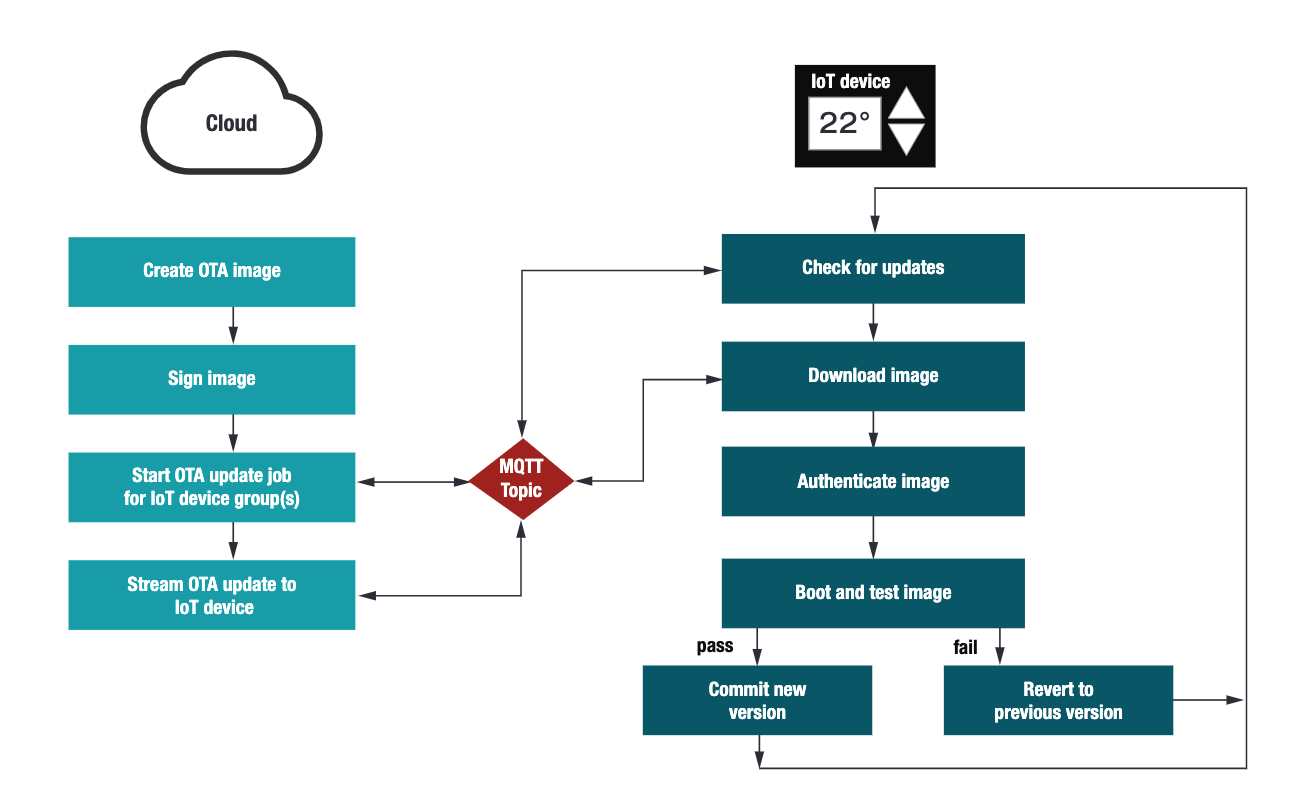
\includegraphics[width=1\textwidth]{gfx/mqtt.png}}
	\caption{MQTT-Protokoll verbindet Cloud mit einem IoT-Gerät}
	\label{fig:mqtt}
\end{figure}

Ein Vorgang für ein OTA-Update mittels eines MQTT-Protokolls ist auf der Abbildung \ref{fig:mqtt} zu sehen \cite[p.5]{website:mqtt}. So verknüpft der OTA-Aktualisierungsdienst die Cloud-Dienste mit einem eingebetteten OTA-Agenten auf dem IoT-Gerät. Sobald ein IoT-Gerät weiß, dass ein Update verfügbar ist, muss es heruntergeladen werden. Ein Ansatz besteht darin, eine Verbindung zu einem dedizierten Server herzustellen und das Update-Image herunterzuladen. Da ein IoT-Gerät in der Regel bereits über einen sicheren Telemetriekanal mit der Cloud verbunden wird, wo das MQTT-Protokoll verwendet wird, kann so das OTA-Update über den MQTT-Kanal heruntergeladen werden. Die Verwendung des MQTT-Kanals ist auch speichereffizienter, da kein HTTP-Client oder ein zusätzlicher TLS-Kanal (Transport Layer Security) erforderlich ist. Um OTA-Update über den MQTT-Kanal sicher herunterladen zu können, muss das Gerät Protokolle wie TLS unterstützen und zunächst eine sichere Verbindung herstellen \cite[p.3]{website:mqtt}.

Da ein zentraler Broker zum effektiven Sammeln und Übertragen von Daten verwendet wird, kann es auf hoch belasteten Verkehrskanälen zu langen Übertragungsverzögerungen kommen, wenn zu viele IoT-Geräte mit dem Broker verbunden sind. Zwar ist das MQTT-Protokoll auf die Gerätekommunikation ausgerichtet, es fehlt jedoch eine IoT-Geräteverwaltungsfunktion. Über Geräteverwaltungssoftware können alle Geräte gewartet und überwacht werden, wie z.B. Software- und Firmware-Updates oder Remote-Konfigurationen. Die Verwendung von Standardprotokollen bietet die Möglichkeit, mit der Verwaltungsplattform anderer Anbieter zu interagieren und weiterhin dieselben nicht standardmäßigen IoT-Geräte verschiedener Marken in Kombination mit Geräten und Standardprotokollen zu verwenden, wodurch Hersteller-Sperren vermieden werden können.


\section{LwM2M und OMA DM-Standards}
\label{sec:ota:oma-dm}
LightweightMachine-to-Machine-Protokoll (LwM2M) wird zur Datenübertragung verwendet und mit DTLS gesichert. Die LwM2M-Spezifikationen definieren ein einfaches Datenmodell und mehrere RESTful-Schnittstellen für die Fernverwaltung von IoT-Geräten. Über die Schnittstellen können sich Geräte bei einem Server registrieren, Informationen aktualisieren und Schlüsselmaterial abrufen. Eine große Anzahl von Objekten und Ressourcen wurde bereits standardisiert, um häufig verwendete Sensoren, Aktoren und andere Ressourcen zu unterstützen. OMA-DM ist von der Open Mobile Alliance entwickelt und eignet sich für Geräte in Bewegung mit Änderung der IP-Adresse und mobile Anwendungen. OMA Lightweight M2M (LwM2M) ist ein leichtes, schnelles und strukturiertes Protokoll, das sich ideal für Geräte mit geringer Kapazität eignet. OMA DM ist ein offenes Protokoll, das im Wesentlichen eine Konfigurationsschicht (wie die API-Schicht) ist. Der OMA DM-Client kommuniziert mit dem Server über HTTPS und verwendet DM Sync (OMA DM v1.2) als Nachrichtennutzlast. Die Spezifikationen für den OMA-DM sind für die Verwaltung von drahtlosen Geräten wie Smartphones, PDAs, Laptops und Tablets vorgesehen. Nachdem der Aufbau der Kommunikation zwischen dem Client und dem Server festgelegt wurde, wird eine Folge von Nachrichten gesendet und somit wird die Information ausgetauscht, um die vom Geräte-Manager gegebene Aufgabe abzuschließen. Einige Warnmeldungen können von OMA-DM außerhalb der Sequenz ausgeführt werden und dienen dazu, Fehler zu behandeln und/oder zu beheben und abnormal Zuständen zu beenden.

Das OMA DM 2.0-Protokoll wird im Kontext einer DM-Sitzung ausgeführt. DM-Sitzungen werden immer vom DM-Client initiiert. Ein DM-Server kann den DM-Client jedoch dazu veranlassen, eine DM-Sitzung zu initiieren, indem er die DM-Benachrichtigung an den DM-Client sendet. Sobald eine DM-Sitzung eingerichtet wurde, sendet der DM-Server die DM-Befehle dem DM-Client und empfängt von ihm Antworten. Der DM-Client informiert den DM-Server auch über generische Warnungen von Ereignisse, die auf dem Gerät aufgetreten sind. Nur der DM-Server sendet DM-Befehle an den DM-Client, und der DM-Client kann keine DM-Befehle senden. Der DM-Server beendet die DM-Sitzung, indem er den Befehl END an den DM-Client sendet \cite[p.13]{website:OMADM}.

\begin{figure}[h!]
	\centering
	\fbox{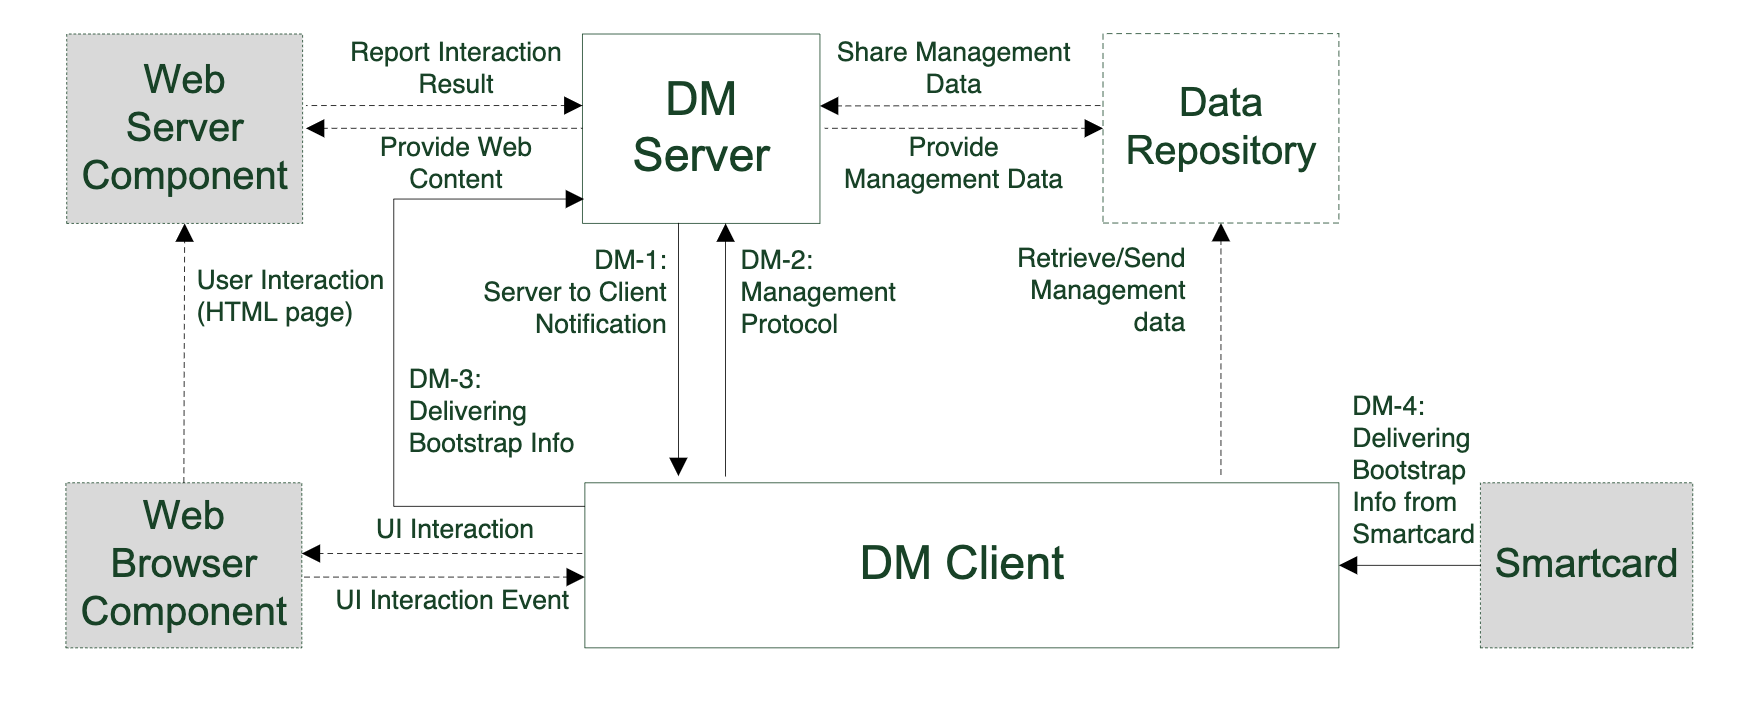
\includegraphics[width=1\textwidth]{gfx/oma_arch.png}}
	\caption{OMA DM Architekturdiagramm}
	\label{fig:oma_arch}
\end{figure}

DM Geräteverwaltung ist der Begriff für Technologie, mit der Dritte die komplizierten Verfahren zum Konfigurieren von Geräten im Auftrag des Endbenutzers (Kunden) ausführen können. Dritte sind in der Regel Betreiber, Dienstleister oder Abteilungen für das Management von Unternehmensinformationen. Durch die Geräteverwaltung kann eine externe Partei Parameter einstellen, Fehlerbehebung bei Terminals durchführen, Software installieren oder aktualisieren \cite[p.7]{website:OMADM2}. Ein OMA DM Architekturmodell ist auf der Abbildung \ref{fig:oma_arch} zu sehen \cite[p.9]{website:OMADM2}.  Der DM-Client und der DM-Server sind die abstrakte Softwarekomponente. Das Datenrepository ist ein logischer Server, und der DM-Client kann Verwaltungsdaten mithilfe von HTTP-Methoden oder anderen Transportprotokollen abrufen und an diese Komponente senden. Der DM-Server kann die Verwaltungsdaten mit dieser Entität austauschen \cite[p.10]{website:OMADM2}.

\section{DM vs MQTT: Unterschiede}
\label{sec:ota:diff}
Es sind sowohl MQTT als auch LwM2M/OMA DM als Standardprotokolle für den Transport von Daten von Geräten zu anderen Geräten, Systemen, Plattformen und Anwendungen geeignet. Während Lightweight M2M speziell für die Geräteverwaltung im Internet der Dinge entwickelt wurde, ist der Telemetrietransport in der Nachrichtenwarteschlange im Wesentlichen ein Publish / Subscribe-basiertes Kommunikationsprotokoll, das Daten und proprietäre DM-Nutzdaten im IoT erfolgreich unterstützen kann. Dies ist besonders wichtig im Zusammenhang mit der Protokollfunktionalität: LwM2M verfügt über ein genau definiertes Daten- und Kommunikationsmodell, das eine Vielzahl gebrauchsfertiger Standardobjekte (OMNA, IPSO, GSMA-Objekte), Konnektivitätsüberwachung, Remote-Geräteaktionen und strukturierte FOTA- und SOTA-Updates, während diese Funktionen in MQTT vollständig hersteller- und plattformspezifisch sind. Was folgt ist, dass mit MQTT Firmware-Updates oder andere Verwaltungsfunktionen von Grund auf neu erstellt werden müssen.

Wenn es um Sicherheit geht, bietet MQTT offensichtlich keine integrierten Sicherheitsfunktionen, kann jedoch bei Bedarf sogar das vollständige TLS-Protokoll verarbeiten (was jedoch den Netzwerkaufwand erheblich erhöht und zu drastischen Kompromissen bei Geschwindigkeit, Leichtigkeit und Funktionalität führt). Während LwM2M ähnliche Funktionen in Bezug auf die Sicherheit der Transportschicht bietet (die die Protokolle DTLS 1.2+ und TLS 1.2+ nativ unterstützen), gewährleistet es durch die Verwendung von OSCORE zusätzlich die Sicherheit der gesamten Anwendungsschicht. Es muss hinzugefügt werden, dass die Verwendung von Sicherheitsfunktionen die Leistung des LwM2M-Protokolls nicht beeinträchtigt.

%\begin{lstlisting}[caption={[XML-Datei für VendorId und ProductID] },captionpos=b]
%/usr/lib/pcsc/drivers/ifd-ccid.bundle/Contents/info.plist
%\end{lstlisting}